\documentclass{beamer} 
%\title{text}
%\author{text}
%\date{date}

\usepackage{tikz}
\usetikzlibrary{mindmap,trees}
\usepackage{verbatim}
\usepackage{adjustbox}

\begin{document}
\begin{frame}
	\titlepage
\end{frame}

\begin{frame}{TITLU FRAME}

\begin{itemize}
	\item The body
	\pause
	\item ALt body
	\pause
	\item altu
\end{itemize}

\end{frame}

\begin{frame}
\begin{adjustbox}{max totalsize={.9\textwidth}{.7\textheight},center}
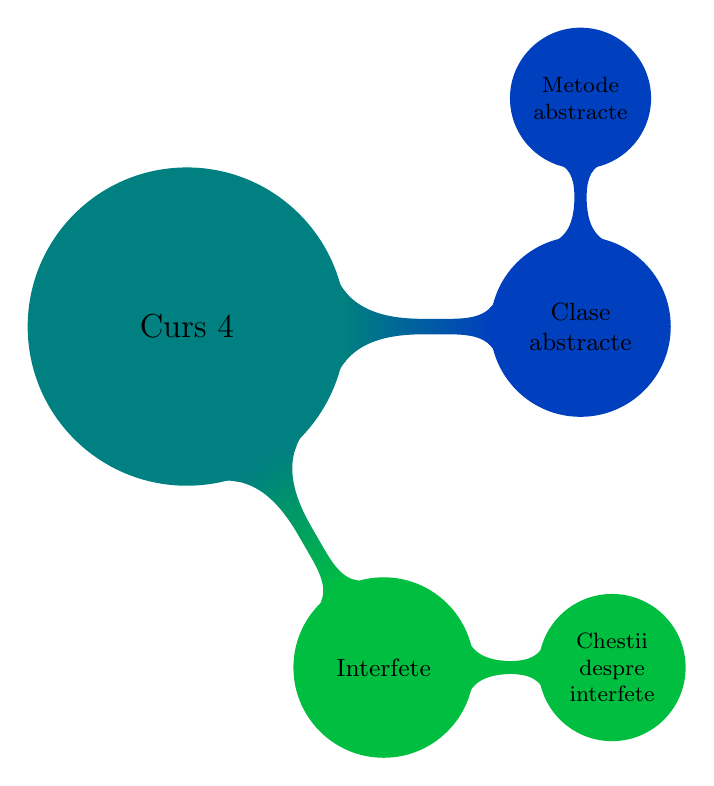
\begin{tikzpicture}
 	\path[mindmap, concept color=teal,text=black]
	node[concept] {Curs 4} [clockwise from=0]
	child[concept color = blue!50!teal] {
		node[concept] {Clase abstracte} [clockwise from=90] 
			child{node[concept] {Metode abstracte} }
}
	child[concept color = green!50!teal] {
		node[concept] {Interfete} [clockwise from=0] 
			child{node[concept] {Chestii despre interfete} }			
}
;
\end{tikzpicture}
\end{adjustbox}
\end{frame}
\end{document}

